\subsection{Gas ideali}
Un gas ideale è costituito da particelle puntiformi, che non abbiano un proprio volume, e contenute in un recipiente in cui è praticato il vuoto in modo da avere solo poche particelle del gas e dove abbiamo dei misuratori di temperatura e pressione.

Definiamo un gas "ideale" quando esso si trova a bassa pressione, quindi rarefatto e ad alta temperatura.

In queste condizioni è ragionevole assumere che non esistano interazioni fra le varie particelle, per cui esse si muovono in modo del tutto casuale. Qualora dovessero esserci urti, si assume che essi siano perfettamente elastici.

Un gas occupa l'intero volume che trova a sua disposizione ed esercita una pressione dovuta agli urti delle particelle del gas sulle superfici interne del recipiente che lo contiene.

Le proprietà di un gas sono determinate dalla sua pressione e dalla sua temperatura.

\vspace{0.2cm}La pressione, cioè la forza esercitata sulle pareti, ha come unità di misura l'\textit{atmosfera} ($atm$). Inoltre $1 \; atm=760 \; mmHg=1 \; Torr$. Nel S.I. l'unità di misura è il \textit{Pascal} ($Pa$), per cui

$$P=N/m^2=\big[ (kg \cdot m)/s^2 \big]/m^2=(kg \cdot m)/(s^2 \cdot m^2)$$
$$\implies P=kg/(s^2 \cdot m)$$

Spesso nelle bombole l'unità di misura è il \textit{bar}. 1 bar equivale a $10^5 \; Pa$.

La temperatura si misura in gradi centigradi (°C) o in gradi Kelvin (K). Per passare da Celsius a Kelvin aggiungiamo 273.15:

$$T(K)=T(^{\circ}C) + 273.15$$
\subsection{Significato molecolare della pressione}
La pressione è dovuta agli urti delle particelle contro le pareti del recipiente che lo contiene ed è la stessa in tutti i suoi punti.
\subsection{Significato molecolare della temperatura}
Supponiamo di avere un gas dentro un contenitore chiuso e di riscaldarlo mantenendo costante il suo volume. Ci accorgiamo che aumenta la pressione, cioè aumenta il numero di urti delle particelle nell'unità di tempo. Se aumentano gli urti, aumenterà la velocità delle particelle. Dalla teoria cinetica molecolare sappiamo che l'energia cinetica di una particella è pari a $E_k=3/2 k_bT$, dove $k_b$ è la costante di Boltzmann e $T$ è la temperatura.

\comment{\hspace{0.5cm}\begin{minipage}{0.55 \textwidth}
    \begin{figure}[H]
        \includegraphics[width=8cm]{immagini/velocità_molecolare.png}
    \end{figure}
\end{minipage}
\begin{minipage}{0.4 \textwidth}
\vspace{0.6cm}Consideriamo l'O$_2$. Notiamo che a 25° C la porzione di molecole che ha velocità elevata è ristretta, mentre a 1000° C tale porzione è molto maggiore.

Deduciamo che aumentare la temperatura significa aumentare la velocità media della maggior parte delle particelle e aumentare la porzione di particelle che hanno velocità molto elevate.
\end{minipage}}

\begin{figure}[H]
    \centering
    \includegraphics[width=8cm]{immagini/velocità_molecolare.png}
\end{figure}

Consideriamo l'O$_2$. Notiamo che a 25° C la porzione di molecole che ha velocità elevata è ristretta, mentre a 1000° C tale porzione è molto maggiore.

Deduciamo che aumentare la temperatura significa aumentare la velocità media della maggior parte delle particelle e aumentare la porzione di particelle che hanno velocità molto elevate.

\subsection{Legge di Boyle}
Se manteniamo costante la temperatura (trasformazione isoterma), il prodotto $P \cdot V$ è costante.

Se quindi il gas subisce $n$ trasformazioni isoterme varrà

$$P_0V_0=P_1V_1=P_2V_2=\ldots=P_nV_n$$

con $P_0$ e $V_0$ condizioni iniziali del gas.

\begin{figure}[htp]
    \centering
    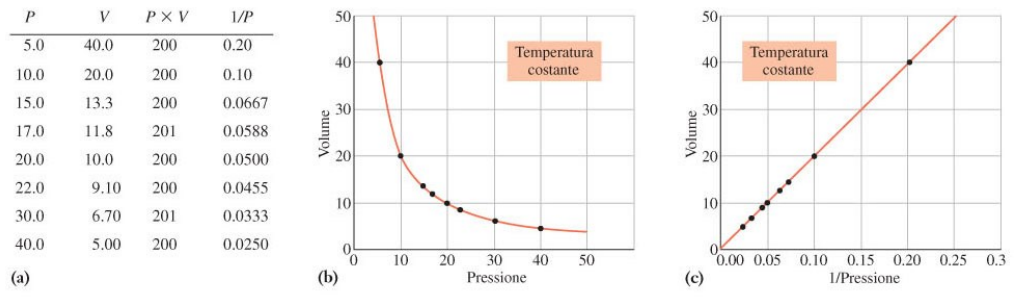
\includegraphics[width=15cm]{immagini/Legge_di_Boyle.png}
\end{figure}

La legge può essere espressa come

$$PV=k \qquad P=\frac{k}{V} \qquad V=\frac{k}{P} \qquad \log{V} = \log{k} - \log{P}$$

\subsection{Legge di Charles (Gay-Lussac)}
Se manteniamo costante la pressione (trasformazione isobara), il volume di un gas aumenterà rispetto a quello iniziale di un 273-esimo per ogni grado di aumento di temperatura:
$$P=cost \implies V_t=V_0(1 + \alpha t), \; \text{con} \; \alpha=\frac{1}{273}$$
$$\implies V_t=V_0 \left( \frac{273 + t}{273} \right), \; T=273 + t$$
$$\implies V_T = \frac{V_0 T}{273}, \; \frac{V_T}{T}=\frac{V_0}{273}=cost$$

E se la temperatura $T$ fosse pari a zero? Sarà zero anche il volume? No, in quanto nella pratica si ha la liquefazione del gas, cioè il volume diminuisce drasticamente perché si ha il liquido.

\vspace{0.2cm}Consideriamo ora un becher con acqua e ghiaccio (immaginiamo di essere a 0° C) nel quale è messa una provetta che al suo interno ha aria. Introduciamo nella provetta alcune goccioline di mercurio (usiamo il mercurio perché può salire e scendere facilmente dato che è un liquido) in modo tale da formare un tappo di mercurio che comprime l'aria fino ad un certo punto per poi quindi bloccarsi.

\begin{figure}[htp]
    \centering
    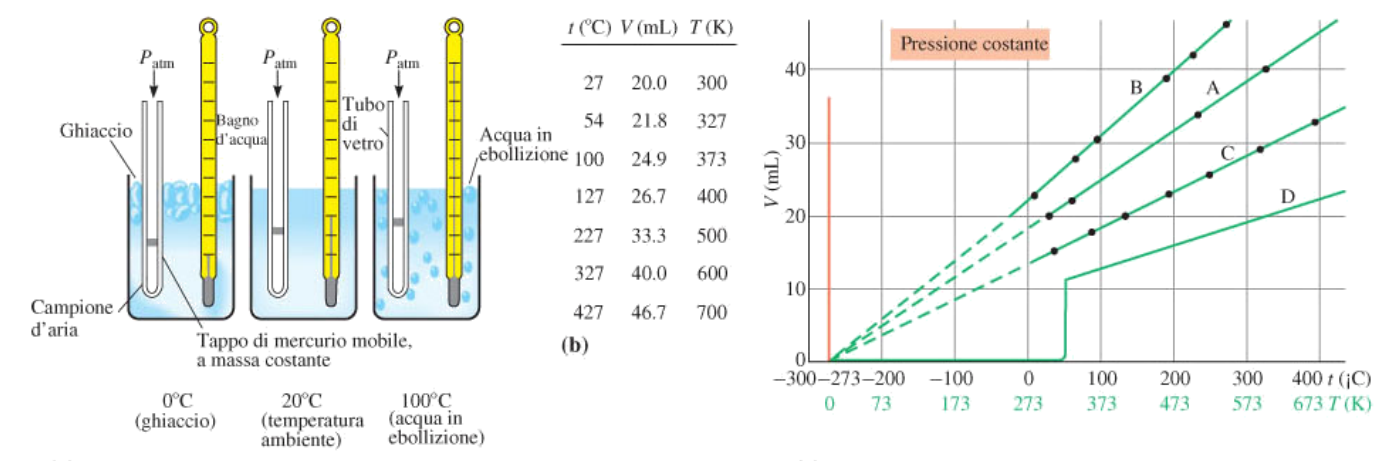
\includegraphics[width=15cm]{immagini/esperimento_provetta.png}
\end{figure}

Se riscaldiamo il sistema ci accorgiamo che il tappo di mercurio si alza, quindi sta cambiando pressione e volume. Se invece oltre a riscaldare manteniamo costante la pressione, noteremo che il volume cresce linearmente con la temperatura. Gli andamenti A, B e C sono quelli dei gas ideali fissati diversi valore di pressione, mentre l'andamento D è quello di un gas reale. In esso notiamo che, andando da destra verso sinistra, a un certo punto il volume crolla. Ciò significa che il gas si è liquefatto, ossia il volume crolla perché il gas si liquefa. Questa è la prova sperimentale che il volume non va a zero.
\subsection{Legge di Gay-Lussac}
Se manteniamo costante il volume (trasformazione isocora) la pressione del gas è proporzionale alla temperatura: per ogni grado di aumento di temperatura la pressione aumenta di 1/273-esimo del suo valore iniziale:

$$V=cost \implies P_t=P_0(1 + \alpha t), \; \text{con} \; \alpha=\frac{1}{273}$$
$$\implies P_t=P_0 \left( \frac{273 + t}{273} \right), \; T=273 + t$$
$$\implies P_T = \frac{P_0 T}{273}, \; \frac{P_T}{T}=\frac{P_0}{273}=cost$$

\subsection{Legge di Dalton delle pressioni parziali}
Supponiamo di avere più di un gas ideale nel volume a disposizione. Abbiamo detto che un gas ideale è caratterizzato dall'assenza di interazione fra le particelle, per cui se tutti i gas presenti hanno tale comportamento non ci saranno interazioni fra le varie particelle, ossia ogni gas si comporta come se fosse l'unico presente nell'intero contenitore. Pertanto la pressione totale sarà pari alla pressione dei singoli gas:
$$P_{tot}=P_1 + P_2 + P_3 + \ldots + P_N = \sum_{i=1}^nP_i
\quad\text{Legge di Dalton}$$

Vediamo un esempio numerico:

\vspace{-0.3cm}
\hspace{0.5cm}\begin{minipage}{0.55 \textwidth}
    \begin{figure}[H]
        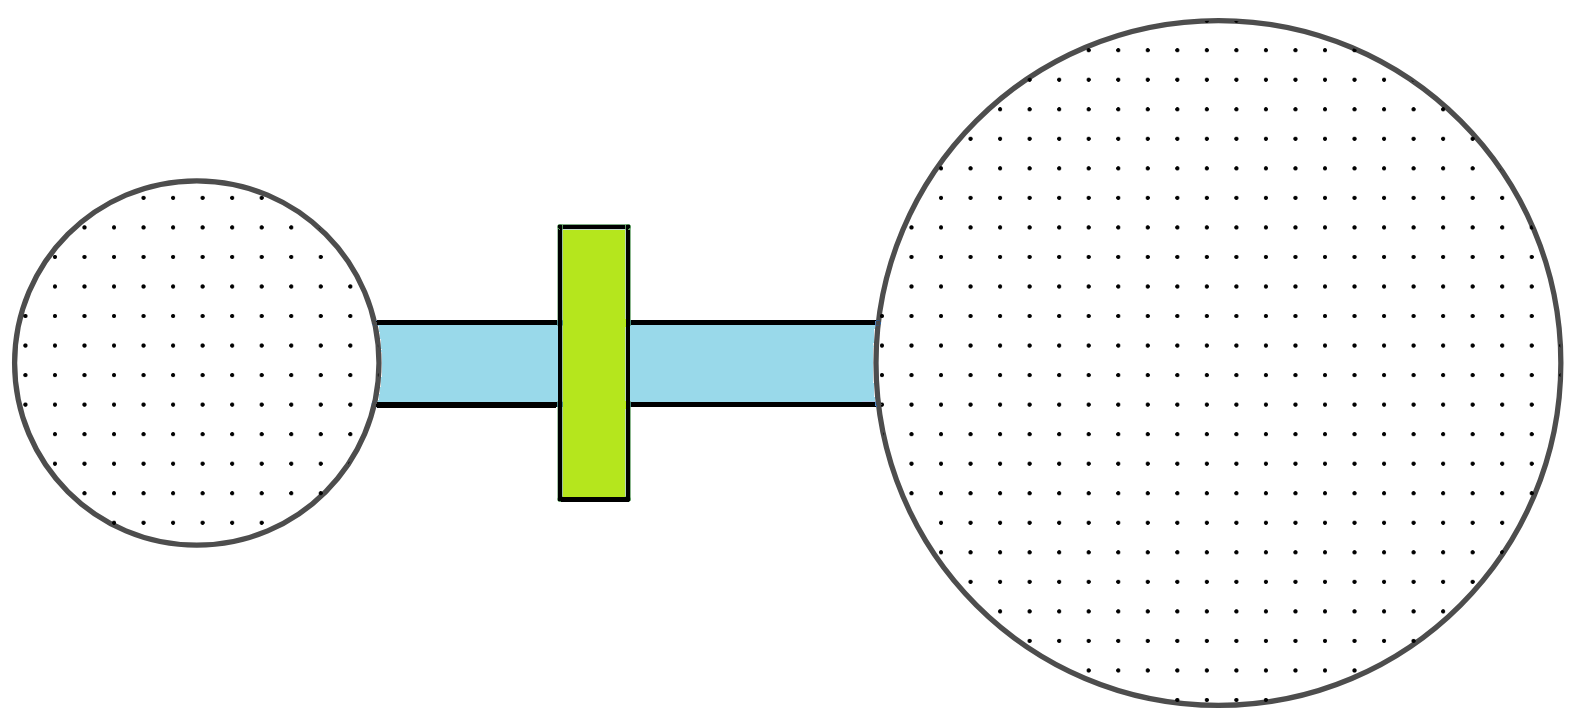
\includegraphics[width=8cm]{immagini/serbatoio.png}
    \end{figure}
\end{minipage}
\begin{minipage}{0.4 \textwidth}
\vspace{0.8cm}Consideriamo due recipienti che hanno al loro interno due gas diversi. Essi inoltre sono collegati con un rubinetto inizialmente chiuso.

Le condizioni iniziali sono

\begin{center}
    \begin{tabular}{p{2.5cm}p{2.5cm}}
        $P_1=175 \; Torr$ & $P_2=125 \; Torr$\\[1ex]
        $V_1=0.527 \; L$ & $V_2=3.141 \; L$
    \end{tabular}
\end{center}
\end{minipage}

\vspace{0.4cm}A temperatura costante vale $PV=cost$.

Il volume finale vale $V_{tot}=V_1 + V_2 =3.668 \; L$

Le pressioni parziali valgono

\vspace{0.2cm}$P_1V_1=P_x \cdot 3.668 \rightarrow 175 \cdot 0.527 = P_x \cdot 3.668 \rightarrow P_x = 25.14 \; Torr$

\vspace{0.2cm}$P_2V_2=P_y \cdot 3.668 \rightarrow 125 \cdot 3.141 = P_y \cdot 3.668 \rightarrow P_y = 107.4 \; Torr$

\vspace{0.2cm}La pressione totale vale $P_{tot}=P_x + P_y=25.14 + 107.04=132.18 \; Torr$. Essa sarà la pressione esercitata dal volume $V_{tot}$, che è calcolata in funzione delle pressioni parziali grazie alla legge di Dalton.
\subsection{Legge dei volumi molari e di Avogadro}
Consideriamo le equazioni
$$\ce{2H_2 + O_2 -> 2H_2O}$$
$$\ce{2CO + O_2 -> 2CO_2}$$
$$\ce{H_2 + Cl_2 -> 2HCl}$$
Esse sono tutte specie gassose.

Sperimentalmente si è visto che, se i gas vengono prelevati nelle stesse condizioni di temperatura e pressione, i rapporti stechiometrici si mantengono anche se anziché considerare moli consideriamo volumi. Dunque, nei nostri esempi, 2 litri di H$_2$ più un litro di O$_2$ daranno luogo a 2 litri di H$_2$O in fase gassosa.

Quindi questi rapporti in moli sono rapporti anche in volumi. Da ciò segue la legge di Avogadro:

\vspace{0.2cm}"\textit{Volumi uguali di gas diversi, nelle stesse condizioni di temperatura e pressione, devono contenere lo stesso numero di molecole. In particolare a 0° C e 1 atm una mole di qualunque gas occupa sempre un volume di} $22.414$ \textit{litri, che è detto volume molare}".

\vspace{0.2cm}Si definiscono \textbf{condizioni normali} 0° C e 1 atm.

\vspace{0.2cm}Si definiscono \textbf{condizioni standard} 25° C e 1 atm.

\vspace{0.2cm}Attenzione! In alcuni testi vengono etichettate, rispettivamente, come \textit{condizioni standard} e \textit{condizioni standard ambientali}. Useremo la prima nomenclatura.
Va da ricordare che una mole contiene $6.023 \cdot 10^{23}$ particelle, tale numero si può determinare così:

Consideriamo il radio. Esso dà luogo per disintegrazione al radon più particelle $\alpha$, le quali sono atomi di elio doppiamente ionizzati:

$$\ce{^{226}_{88}Ra -> ^{222}_{86}Rn + \alpha \; \text{+ energia,} \qquad \alpha= ^{4}_{2}He^{2+}}$$

Sperimentalmente si osservò che in condizioni normali per $1.165 \cdot 10^{18}$ disintegrazioni di radio si ottengono 0.043 mL di elio.

Il rapporto stechiometrico della reazione è 1:1:1, per cui si formeranno un numero di atomi di elio pari al numero di disintegrazioni. Essi occuperanno un volume di 0.043 mL. Quanti ce ne stanno il 22414 mL? Si fa una proporzione:

$$1.165 \cdot 10^{18}:0.043=x:22414 \implies x \approx 6.023 \cdot 10^{23}$$

che è proprio il numero di Avogadro, misurato sperimentalmente.

Abbiamo ottenuto quindi che

\begin{figure}[htp]
    \centering
    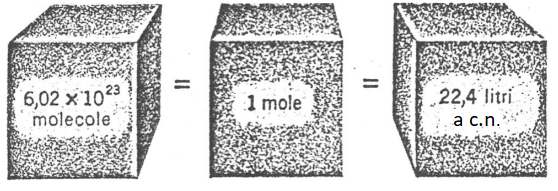
\includegraphics[width=8cm]{immagini/legge_di_avogadro.png}
\end{figure}

cioè abbiamo una relazione diretta tra numero di particelle e volume, pertanto è chiaro che una espressione in moli può diventare un'espressione in volume.
\subsection{Equazione di stato}
$$PV=nRT$$
dove $R$ è la costante universale dei gas. Calcoliamola nel caso $n=1$.

Alla pressione di 1 atm, alla temperatura di 273 K e con un volume di 22.414 L si ottiene

$$n=1 \implies PV=RT \implies R=\frac{PV}{T}=\frac{1 \cdot 22.414}{273}=0.082$$

Dal fatto che tale rapporto sia uguale ad una costante, deduciamo che se il gas subisce una trasformazione e passa da uno stato 1 ad uno stato 2 si avrà

$$\frac{P_1V_1}{T_1}=\frac{P_2V_2}{T_2}$$

Da essa possiamo ricavare le tre leggi viste in precedenza:

\begin{itemize}
    \item Se $T=cost \rightarrow$ legge di Boyle;
    \item Se $P=cost \rightarrow$ legge di Charles;
    \item Se $V=cost \rightarrow$ legge di Gay-Lussac.
\end{itemize}
\subsection{Determinazione dei pesi molecolari}
Supponiamo di avere una sostanza di cui conosciamo la massa ma non sappiamo che sostanza sia. Si può allora usare l'equazione di stato dei gas per calcolare il peso molecolare incognito, il quale è un primo indizio.

L'equazione di stato afferma che $PV=nRT$, ma $n$ è il numero di moli, che si ottiene dividendo la massa per il peso molecolare: $n=g/MM$. Sostituendo nell'equazione di stato troviamo:
$$n=\frac{g}{MM} \implies PV=\frac{g}{MM}RT \implies MM=\frac{g \cdot RT}{PV}$$
Moltiplichiamo entrambi i termini per $MM$:
$$PV \cdot MM=\frac{g}{MM}\cdot MM RT \implies PV MM = gRT$$
$$ \implies PMM = \frac{g}{V}RT, \quad d=\frac{g}{V} \; \text{(densità)}$$
$$\implies MM = d \frac{RT}{P}$$
\subsection{Gas reali}
Nello studio dei gas ideali abbiamo supposto che

\begin{itemize}
    \item Le loro particelle siano in rapido e casuale movimento, non interagendo tra loro:
    \item Tali particelle siano puntiformi, cioè non posseggano volume proprio.
\end{itemize}

\E chiaro che tale gas non può esistere. In un gas reale infatti le particelle:

\begin{itemize}
    \item Non sono puntiformi;
    \item Hanno volume proprio;
    \item Interagiscono tra loro. 
\end{itemize}

Infatti noi riusciamo a far diventare un gas un vapore per poi liquefarlo, cosa che implica l'esistenza di interazioni, addirittura le particelle si legano tra loro per formare un liquido, per cui devono esistere delle forze attrattive tra le particelle.

Ciononostante, se ci mettiamo in condizioni di bassa pressione (entro le 100 atm) e alta temperatura i gas mostrano un comportamento ideale.

Graficamente infatti si ha una tale situazione:

\begin{minipage}{0.55 \textwidth}
    \begin{figure}[H]
        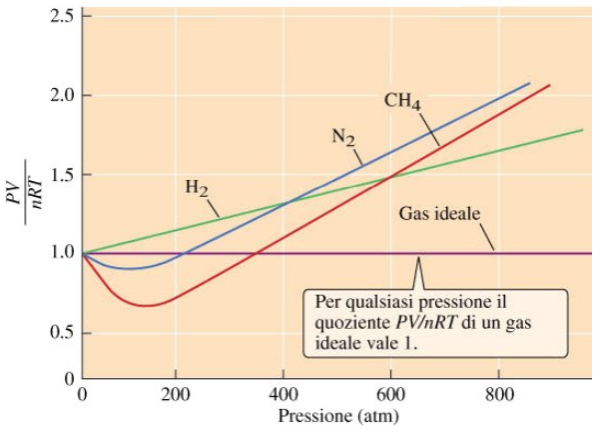
\includegraphics[width=8cm]{immagini/grafico_gas_reali.png}
    \end{figure}
\end{minipage}
\begin{minipage}{0.44 \textwidth}
\vspace{-0.4cm}Se il gas è ideale il rapporto $PV/nRT$, detto \textit{fattore di comprimibilità di un gas} è costantemente uguale a 1, qualunque sia la pressione. 

\vspace{0.2cm}Se invece il gas è reale, tale rapporto vale ancora 1 per pressioni prossime allo zero, ma man mano che la pressione aumenta l'andamento del rapporto si allontana dall'idealità.
\end{minipage}

Cerchiamo di capire cosa succede.

Se siamo ad alte pressioni, tale rapporto è maggiore di 1. Dato che il fattore di comprimibilità sta crescendo, significa che il gas è meno comprimibile rispetto a quanto previsto dalla legge di Boyle. \E meno comprimibile in quanto le particelle sono dotate di volume, mentre nel caso ideale assumiamo non ne abbiano. Il volume del gas infatti non è pari al volume del recipiente, ma a quello del recipiente meno quello occupato dalle singole molecole. Quindi a pressioni alte il gas è meno comprimibile e il volume è maggiore di quello che si calcola per un gas ideale.

A basse pressioni il gas sarà più comprimibile rispetto al valore atteso dalla legge di Boyle, e se le forze attrattive aumentano possiamo anche liquefare il gas. Tale aumento di comprimibilità è dovuto alle forze attrattive, le quali a loro volta sono funzioni della temperatura, per cui se la temperatura è alta queste forze sono meno efficaci, se invece è bassa esse diventano incisive e quindi il volume sarà minore di quello che si osserva per un gas ideale.

Pertanto, mentre a basse pressioni siamo pressoché in condizioni ideali, ad alte pressioni l'equazione di stato non è più valida in quanto vale l'\textbf{equazione di Van der Waals}:

$$\left( P + \frac{n^2a}{V^2} \right)\big(V-nb\big)=nRT$$

Il termine $a/V^2$ tiene conto delle interazioni attrattive tra le particelle, in modo da correggere la pressione. Il volume invece viene corretto sottraendo un termine $b$ detto \textit{covolume} o \textit{volume proprio delle particelle}, in questo modo sottraiamo al volume del contenitore quello delle particelle.

Il parametro $a$ dipende dalle forze attrattive tra le particelle.

Il parametro $b$ dipende dalla dimensione delle particelle.

\vspace{0.2cm}Il volume occupato da una particella non è esclusivamente il volume della particella stessa se la aggreghiamo con altre particelle. In che senso?

\begin{minipage}{0.34 \textwidth}
    \begin{figure}[H]
        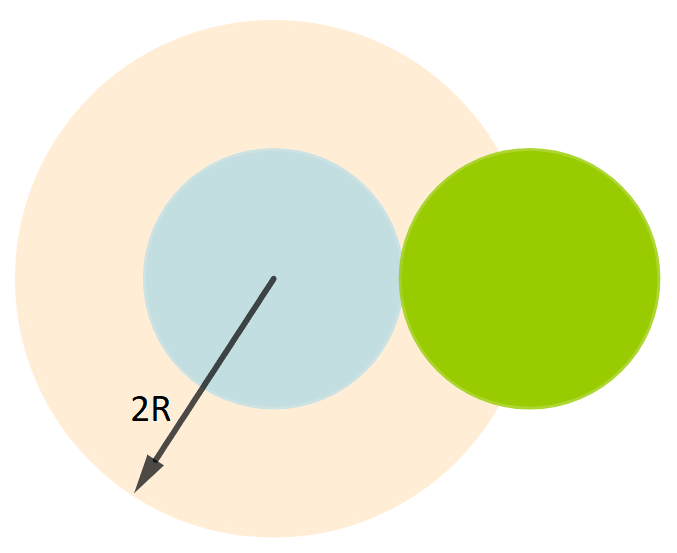
\includegraphics[width=5cm]{immagini/particelle_aggregate.png}
    \end{figure}
\end{minipage}
\begin{minipage}{0.65 \textwidth}
    \vspace{0.8cm}Supponiamo che una data molecola, schematizzata come una sfera di raggio $R$, si trovi a stretto contatto con altre molecole circostanti. Attorno ad essa riusciamo a posizionare altre sei molecole.
    Il centro della molecola data si troverà a distanza 2R dal centro delle molecole adiacenti. Se adesso consideriamo una sfera di raggio 2R troveremo al suo interno, oltre alla data molecola, anche circa la metà di ognuna delle molecole circostanti.
    Il volume che una molecola occupa, precludendolo alle altre molecole, corrisponderà quindi a circa metà del volume di una sfera di raggio 2R. 
\end{minipage}

\vspace{0.2cm}Nel limite di tale approssimazione, ad ogni molecola occorre assegnare un volume:

$$V = \frac{1}{2} \times \frac{4}{3}\pi (2R)^3 = 4 \times \frac{4}{3}\pi R^3$$

Cioè, quattro volte superiore al volume effettivo della molecola, ovvero $b \approxeq 4V_M$.
\subsection{Gas e vapori}
Supponiamo di avere dell'acqua e di riscaldarla fino a 200° C. Essa, raggiunta la temperatura di 100° C, rimarrà a tale temperatura finché tutta l'acqua non passa allo stato di vapore. Dopodiché crescerà la temperatura del vapore.

Cerchiamo quindi di capire la differenza tra vapore e gas:

\vspace{-0.4cm}

\hspace{1cm}\begin{minipage}{0.53 \textwidth}
    \begin{figure}[H]
        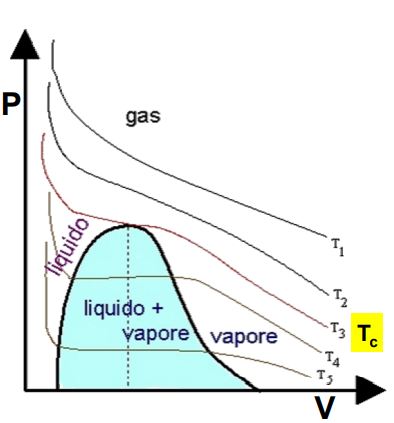
\includegraphics[width=7cm]{immagini/grafico_pV.png}
    \end{figure}
\end{minipage}
\begin{minipage}{0.4 \textwidth}
\vspace{0.6cm}Consideriamo l'andamento di pressione e volume di una certa sostanza gassosa ad una fissata temperatura.

\vspace{0.2cm}Si definisce \textbf{temperatura critica} quella temperatura sopra la quale non è più possibile liquefare un gas, qualunque sia la pressione esercitata su di esso. Pertanto per farlo liquefare dovremo prima portarlo sotto la temperatura critica e poi applicare la giusta pressione.
\end{minipage}

\vspace{0.2cm}Quindi quando si parla di gas intendiamo specie chimiche che siano al di sopra della loro temperatura critica. Se invece fossero al di sotto di questa dovremmo parlare di vapore. In altre parole, se abbiamo un gas non potremo trasformarlo in liquido per compressione, mentre ciò è sempre possibile se abbiamo un vapore.

\vspace{0.2cm} Il diagramma di sopra ci permette di capire in che fase si trova la sostanza, infatti è detto \textbf{diagramma di fase}. In particolare la zona in cui abbiamo sia liquido che vapore è detta \textbf{campana di coesistenza}. Se ci troviamo al suo interno e variamo di poco pressione e volume la coesistenza permane, se invece ci troviamo sulla linea di contorno, non appena variamo la pressione o il volume non siamo più in condizioni di coesistenza e avremo solo una fase.